\begin{figure}[H]
  \centering
  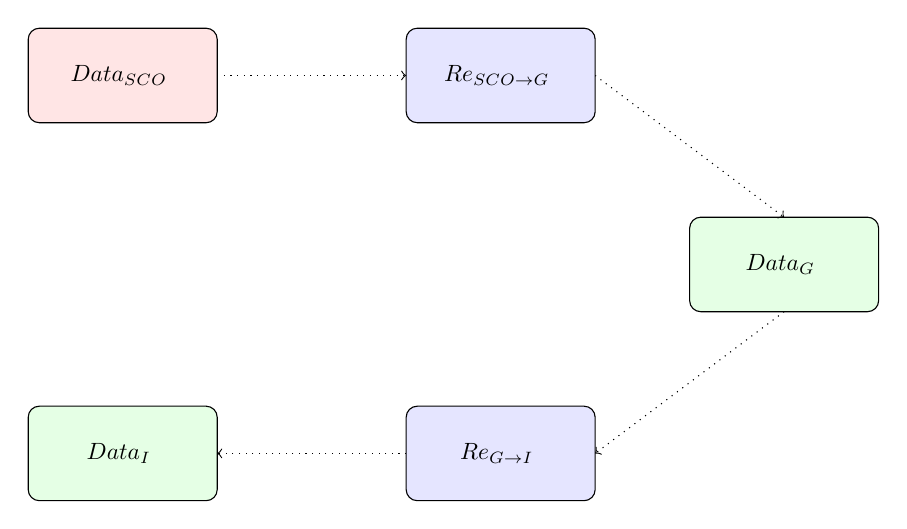
\begin{tikzpicture}[scale = 0.6, every node/.style={scale = 0.85}, every node/.append style={fill = white, rounded corners = 2pt, inner sep = 2pt, align = center}]

  \draw [rounded corners, fill=green!10] (-10, -7) rectangle (-6, -9);
  \node [fill=green!10] at (-8, -8) { $\text{Data}_{\text{I}}$ };

  \draw [ -> , dotted] (-2, -8) -- (-6, -8);

  \draw [rounded corners, fill=blue!10] (-2, -7) rectangle (2, -9);
  \node [fill=blue!10] at (0, -8) { $\text{Re}_{\text{G} \rightarrow \text{I}}$ };

  \draw [ -> , dotted] (6, -5) -- (2, -8);

  \draw [rounded corners, fill=green!10] (4, -3) rectangle (8, -5);
  \node [fill=green!10] at (6, -4) { $\text{Data}_{\text{G}}$ };

  \draw [ -> , dotted] (2, 0) -- (6, -3);

  \draw [rounded corners, fill=blue!10] (-2, 1) rectangle (2, -1);
  \node [fill=blue!10] at (0, 0) { $\text{Re}_{\text{SCO} \rightarrow \text{G}}$ };

  \draw [ -> , dotted] (-6, 0) -- (-2, 0);

  \draw [rounded corners, fill=red!10] (-6, 1) rectangle (-10, -1);
  \node [fill=red!10] at (-8, 0) { $\text{Data}_{\text{SCO}}$ };

  \end{tikzpicture} \\
  \caption{
  	Group Read Re-encryption (theoretical)
  }{
    The theoretical process of re-encrypting from a storage contract owner to a group, then re-encrypting again from the group to an individual (member of the group).
  }
  \label{fig:encryption_group_read_theoretical}
\end{figure}
